\chapter{Analisi Architetturale del Sistema}
\label{chap:analisi_globale}

A conclusione dello sviluppo, è stata condotta un’analisi trasversale per valutare la qualità strutturale del sistema \textit{JarFin} nella sua interezza. L'obiettivo è verificare come i diversi microservizi interagiscano e se l'architettura rispetti i principi di modularità.

\section{Analisi delle Dipendenze}

Il grafico delle dipendenze (Chord Diagram) offre una vista topologica delle interazioni tra i package del sistema.

Le linee di connessione rappresentano le dipendenze dirette tra le classi. Come si evince dalla Figura \ref{fig:main_dependencies}:
\begin{itemize}
    \item I collegamenti sono \textbf{direzionali e ordinati}: il flusso parte dai Controller (blu/azzurro), attraversa i Service (verde) e arriva ai DTO/Modelli (grigio/arancione).
    \item Non vi sono "grovigli" (spaghetti code) che collegano moduli non correlati (es. l'Accounting non accede direttamente ai repository dell'Analytics).
    \item I fasci di linee densi verso i DTO confermano che questi oggetti sono correttamente utilizzati come unico mezzo di trasporto dati tra i layer.
\end{itemize}

\begin{figure}[H]
    \centering
    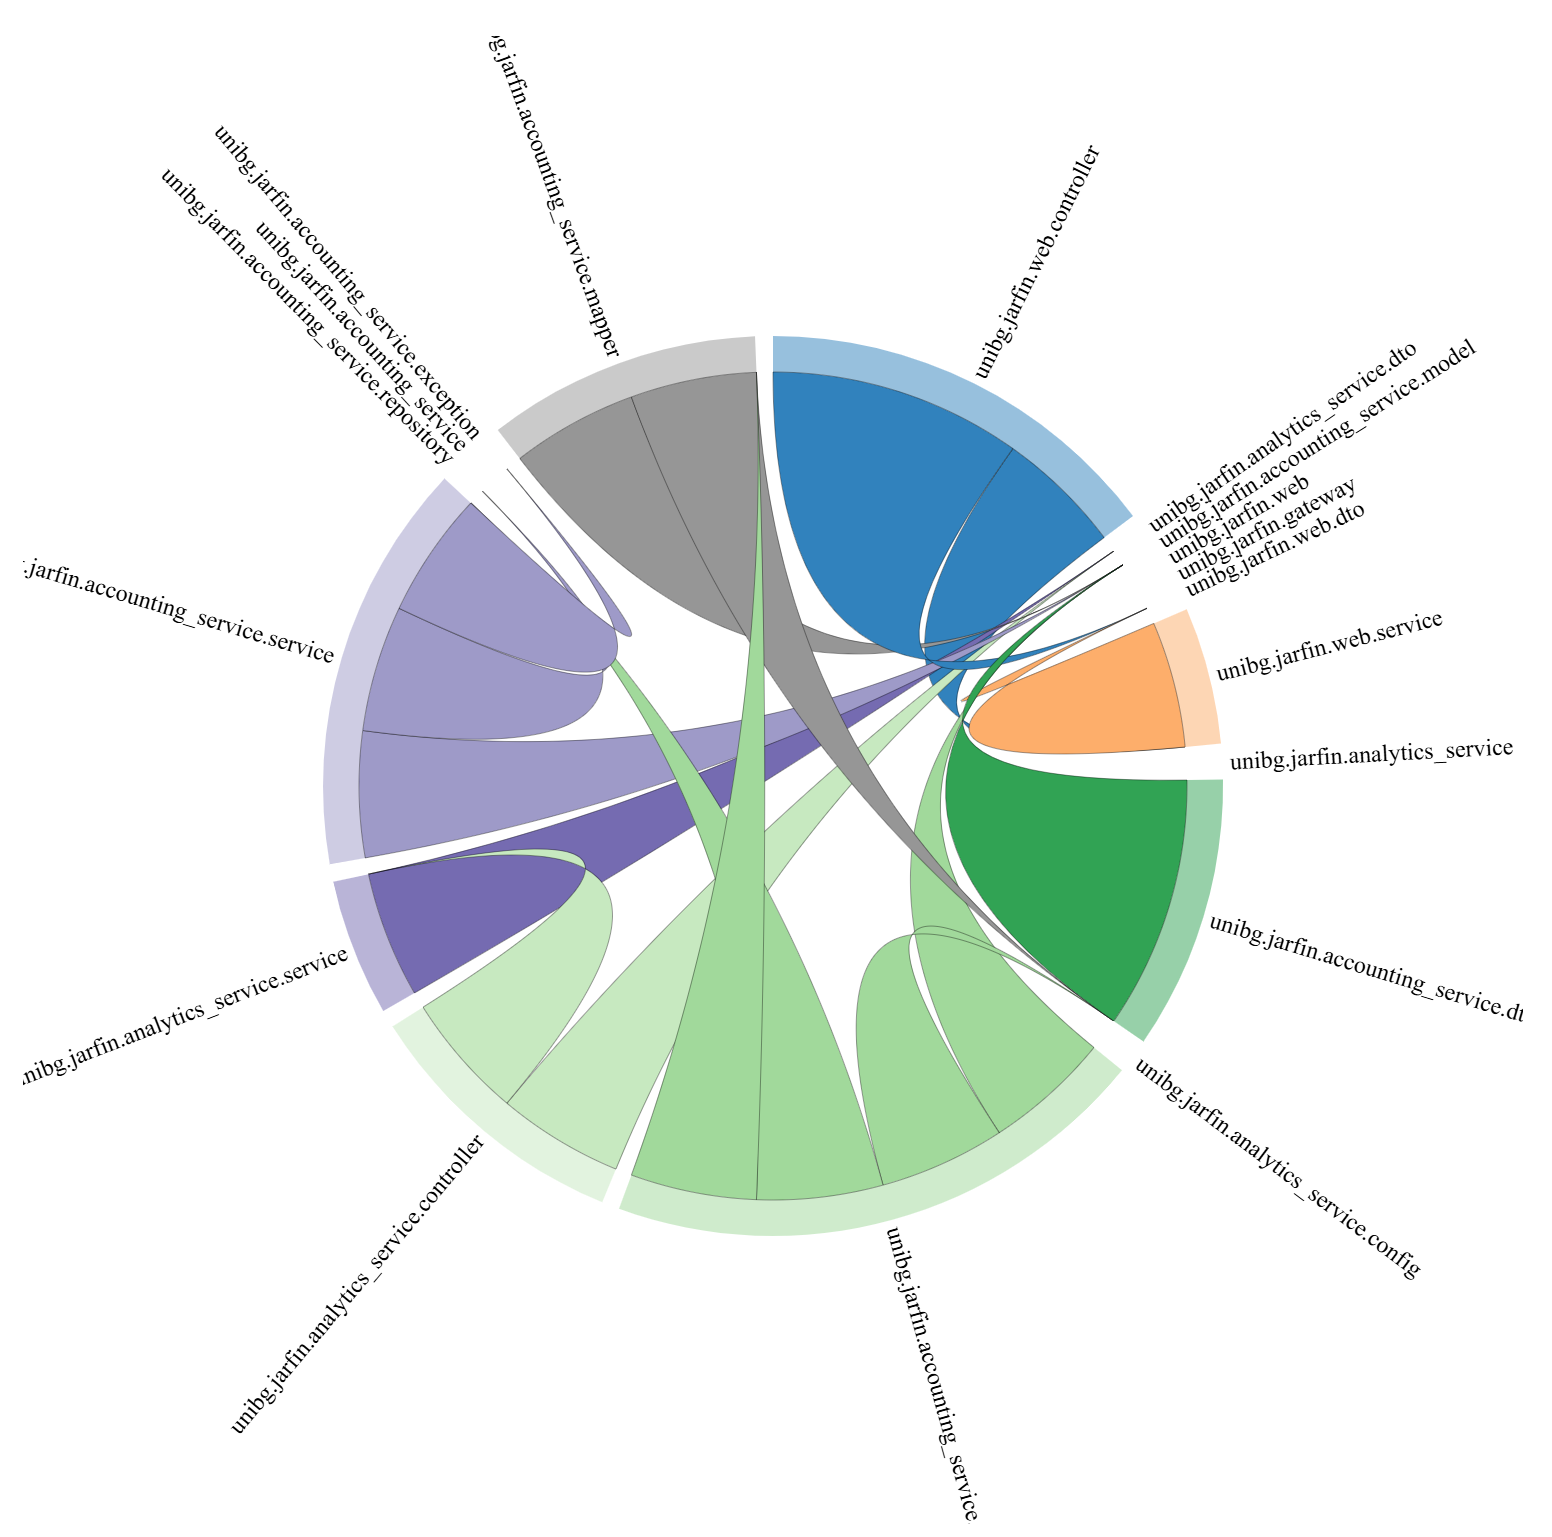
\includegraphics[width=0.77\textwidth]{../3_Images/metriche_JarFin/packages-dependency.png}
    \caption{Grafo delle dipendenze (Chord Diagram) per il sistema JarFin}
    \label{fig:main_dependencies}
\end{figure}

\section{Salute del Codice (Code Health)}

Utilizzando la visualizzazione a bolle (Circle Packing) di CodeMR (Figura \ref{fig:main_coupling}), è possibile valutare a colpo d'occhio la salute del codice basandosi su Accoppiamento (Coupling) e Dimensione.
\begin{itemize}
    \item \textbf{Colore (Accoppiamento):} Il verde predominante indica che la maggior parte delle classi ha poche dipendenze verso l'esterno (\textit{Low Coupling}), rendendo il sistema facile da manutenere. L'unica "bolla" gialla rilevante è il \texttt{Web Controller}: questo è un comportamento atteso e corretto, poiché agisce da Orchestratore/Gateway e deve necessariamente conoscere molti altri componenti per coordinarli.
    \item \textbf{Dimensione delle bolle:} La dimensione è proporzionale alla complessità o alle linee di codice. L'omogeneità delle bolle verdi indica una buona distribuzione della logica: non ci sono classi giganti che accentrano troppe funzionalità.
\end{itemize}

\begin{figure}[H]
    \centering
    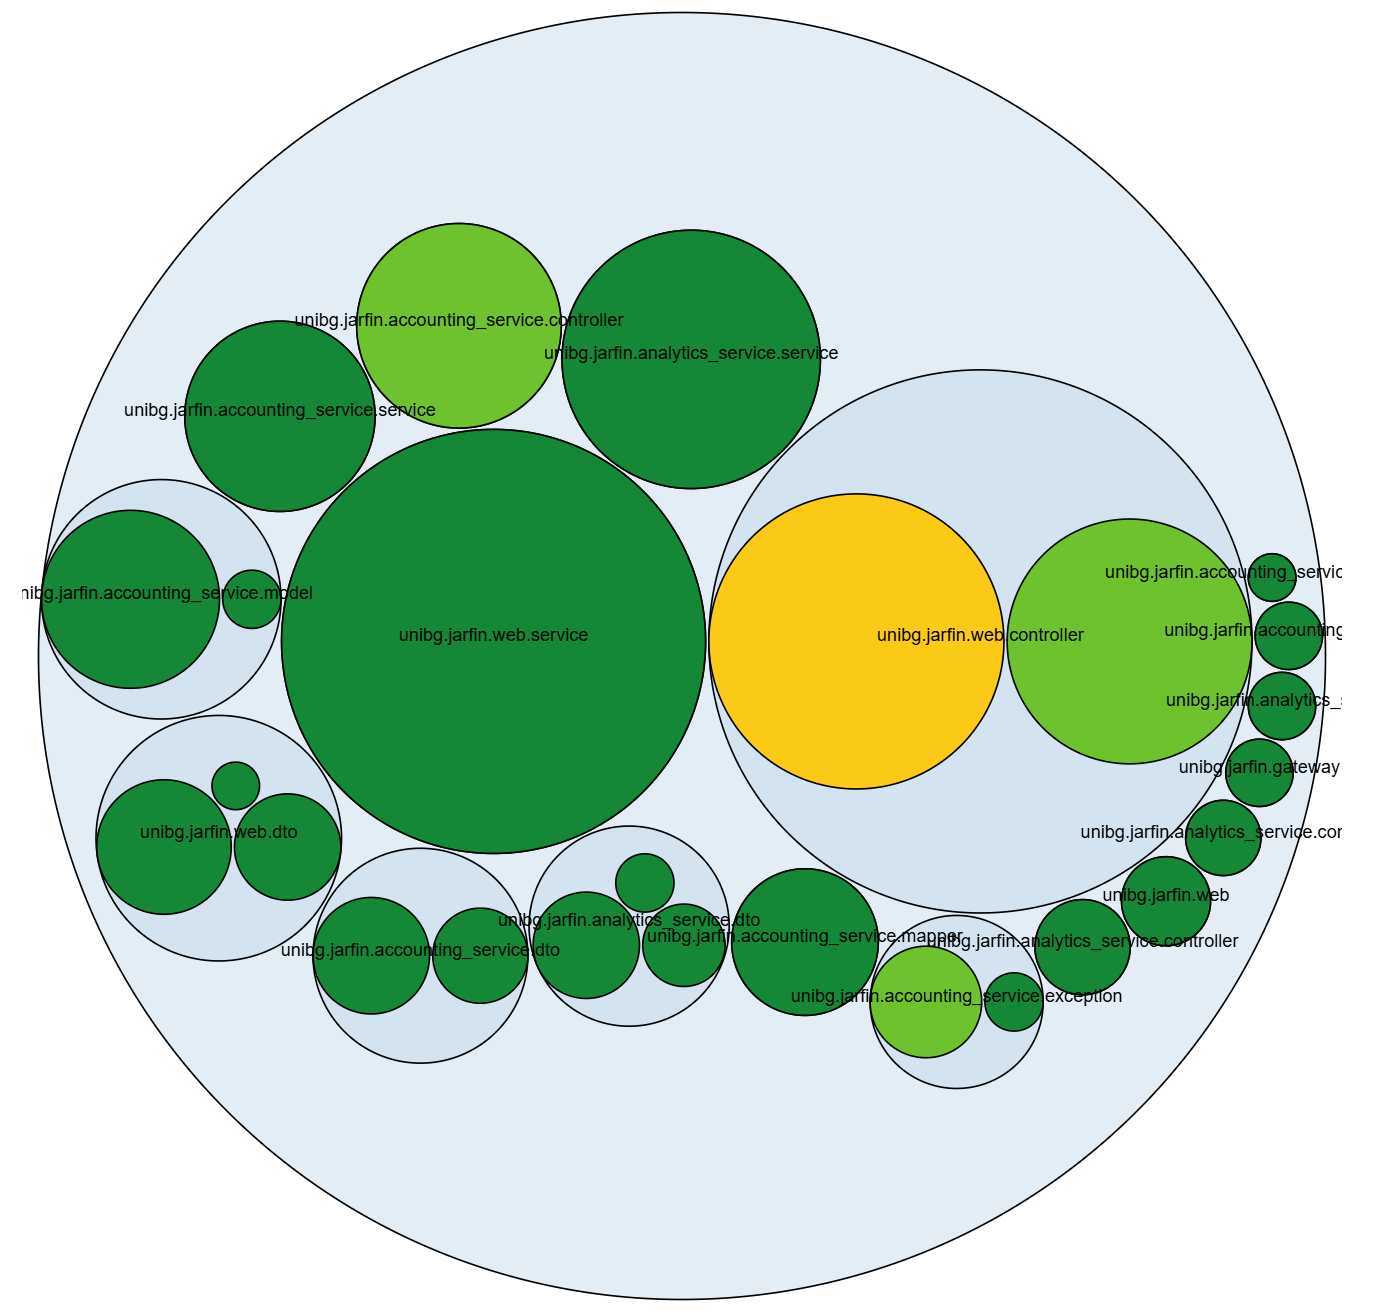
\includegraphics[width=0.8\textwidth]{../3_Images/metriche_JarFin/coupling_between_object_classes.png}
    \caption{Visualizzazione dell'accoppiamento}
    \label{fig:main_coupling}
\end{figure}

\section{Metriche di Dettaglio e Assenza di Anomalie}

Per confermare quantitativamente l'analisi visiva, CodeMR fornisce un report sulle anomalie critiche.
La Figura \ref{fig:main_metrics} mostra quattro barre di stato:
\begin{itemize}
    \item \textbf{Rosso e Arancione (0 classi):} Il sistema non contiene classi con alta complessità o alto accoppiamento.
    \item \textbf{Assenza di God Classes:} Il fatto che le prime due barre siano vuote è il risultato più significativo. Significa che non esistono singole classi che violano il principio di responsabilità singola (SRP), un problema comune nei progetti che crescono rapidamente.
\end{itemize}

\begin{figure}[H]
    \centering
    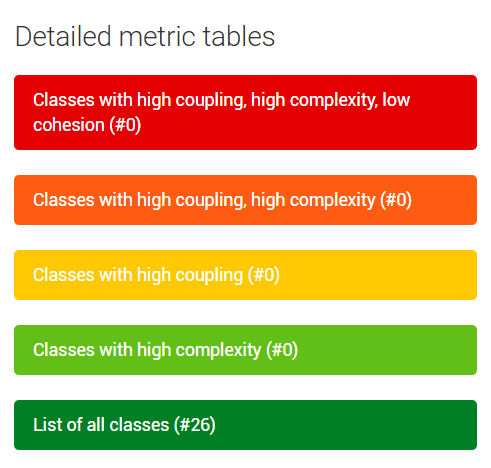
\includegraphics[width=0.7\textwidth]{../3_Images/metriche_JarFin/detailed_metrics.png}
    \caption{Report delle anomalie}
    \label{fig:main_metrics}
\end{figure}

\section{Overview degli Attributi di Qualità}

Infine, i grafici a ciambella (Donut Charts) in Figura \ref{fig:main_quality} offrono una sintesi percentuale dei tre pilastri della qualità software:

\begin{enumerate}
    \item \textbf{Complexity (Alto a SX):} Oltre il 99\% del codice (somma delle sezioni verdi) ha una complessità bassa o molto bassa. Il codice è leggibile e lineare.
    \item \textbf{Coupling (Alto a DX):} Circa l'87\% delle classi ha un accoppiamento basso o medio-basso. Solo il 13.2\% (la sezione gialla) ha un accoppiamento medio, giustificato dai Controller di coordinamento.
    \item \textbf{Lack of Cohesion (Basso a SX):} L'84.5\% delle classi ha una coesione alta (il grafico misura la \textit{mancanza} di coesione, quindi il verde indica "bassa mancanza", ovvero "alta coesione"). I metodi all'interno delle classi sono fortemente correlati tra loro.
\end{enumerate}

\begin{figure}[H]
    \centering
    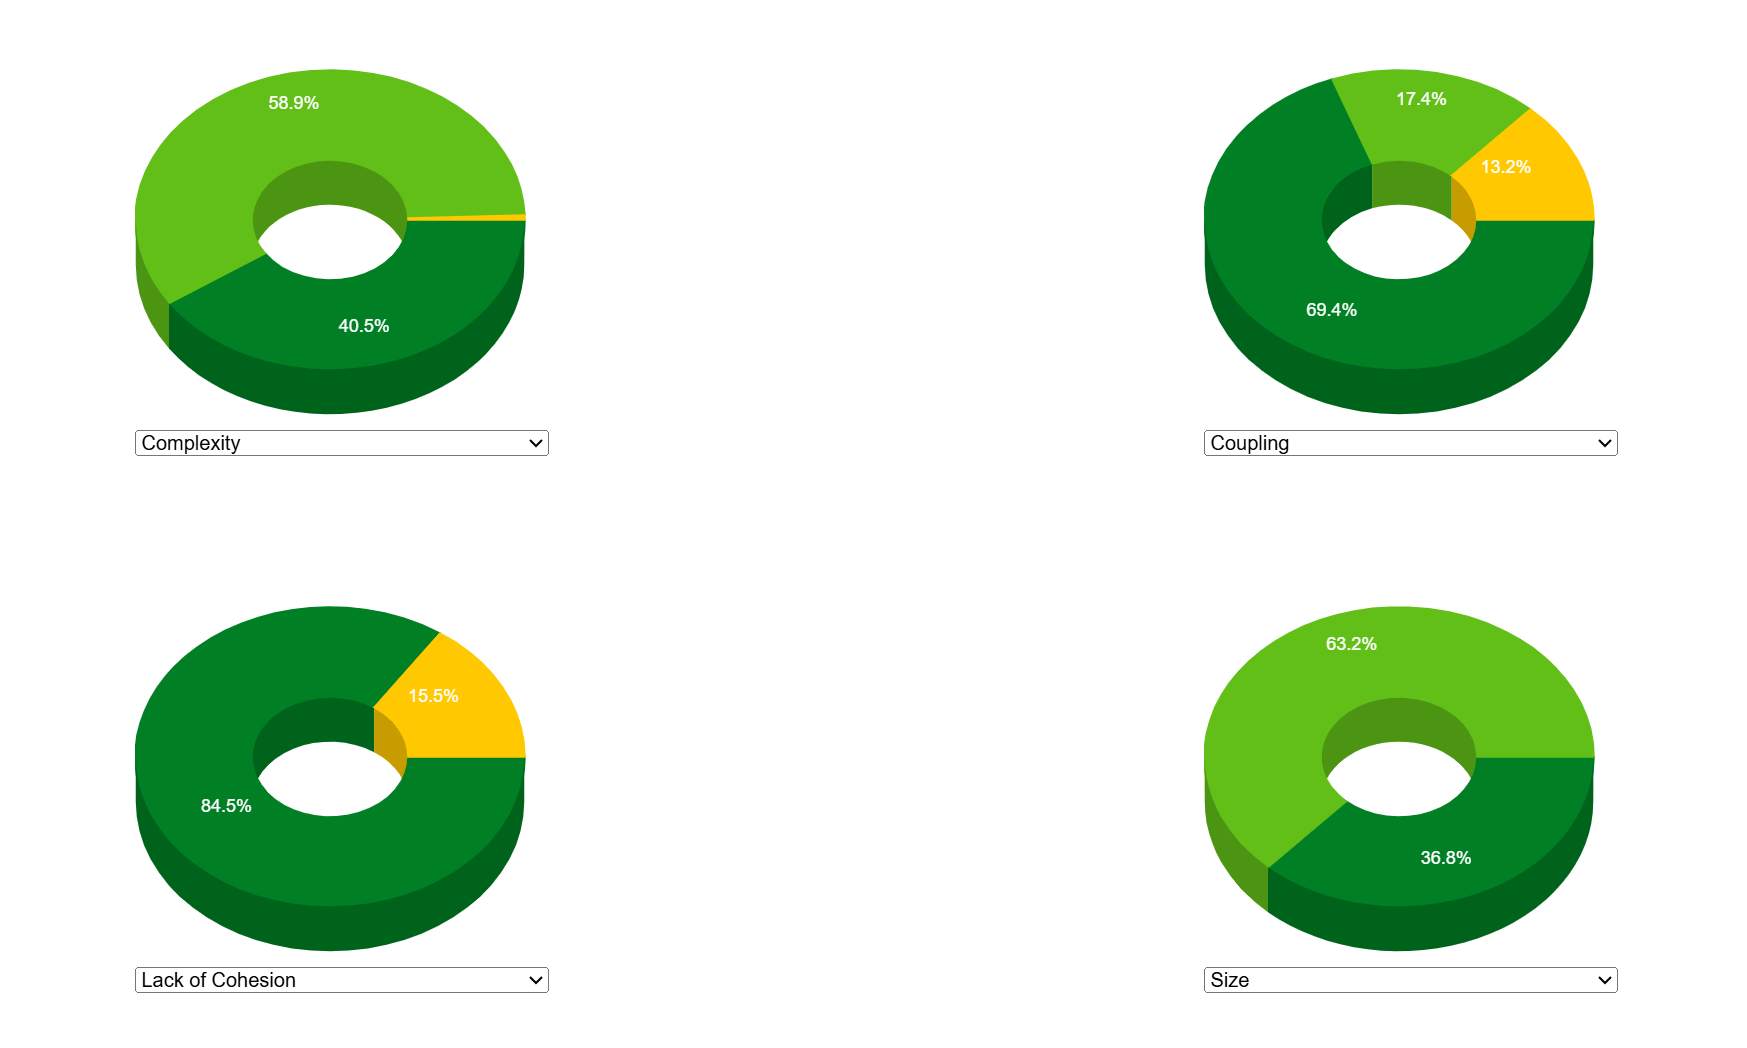
\includegraphics[width=1\textwidth]{../3_Images/metriche_JarFin/quality-attributes.png}
    \caption{Overview percentuale: Complessità, Accoppiamento e Coesione}
    \label{fig:main_quality}
\end{figure}